\documentclass[10pt,a4paper,twocolumn,twoside]{article}
\usepackage[utf8]{inputenc}
\usepackage[english]{babel}
\usepackage{multicol}
\usepackage{graphicx}
\usepackage{fancyhdr}
\usepackage{times}
\usepackage{titlesec}
\usepackage{multirow}
\usepackage{lettrine}
\usepackage{pdflscape}
\usepackage[edges]{forest}
\usepackage{url}
\usepackage[top=2cm, bottom=1.5cm, left=2cm, right=2cm]{geometry}
\usepackage[figurename=Fig.,tablename=TAULA]{caption}
\captionsetup[table]{textfont=sc}

\author{\LARGE\sffamily Segovia Barreales, Richard}
\title{\Huge{\sffamily Reducing dizziness when using a video-see-through head-mounted display}}
\date{}

\newcommand\blfootnote[1]{%
  \begingroup
  \renewcommand\thefootnote{}\footnote{#1}%
  \addtocounter{footnote}{-1}%
  \endgroup
}

%
%\large\bfseries\sffamily
\titleformat{\section}
{\large\sffamily\scshape\bfseries}
{\textbf{\thesection}}{1em}{}

\begin{document}

\fancyhead[LO]{\scriptsize AUTHOR: SEGOVIA BARREALES, RICHARD}
\fancyhead[RO]{\thepage}
\fancyhead[LE]{\thepage}
\fancyhead[RE]{\scriptsize EE/UAB TFG INFORMÀTICA: REDUCING DIZZINESS WHEN USING A VIDEO-SEE-THROUGH HEAD-MOUNTED DISPLAY}

\fancyfoot[CO,CE]{}

\fancypagestyle{primerapagina}
{
   \fancyhf{}
   \fancyhead[L]{\scriptsize TFG EN ENGINYERIA INFORMÀTICA, ESCOLA D'ENGINYERIA (EE), UNIVERSITAT AUTÒNOMA DE BARCELONA (UAB)}
   \fancyfoot[C]{\scriptsize March 2018, Escola d'Enginyeria (UAB)}
}

\renewcommand{\headrulewidth}{0pt}
\renewcommand{\footrulewidth}{0pt}
\pagestyle{fancy}

\maketitle

\thispagestyle{primerapagina}


\blfootnote{$\bullet$ E-mail: richard.segovia@e-campus.uab.cat}
\blfootnote{$\bullet$ Menció en Computació}
\blfootnote{$\bullet$ Project supervised by: Coen Antens (CVC) and Felipe Lumbreras (Computació)}
\blfootnote{$\bullet$ Course 2017/18}

\section{Introduction}

\lettrine[lines=3]{L}{ast} summer during my internship I developed a basic video-see-through viewer for a head mounted display (HDM) prototype developed in the CVC\footnote{Computer Vision Center located in the UAB campus.}, the main goal is to improve this viewer making it expandable for future modules and reduce the adverse physical reactions that it can produce to the users \cite{disconfortReview}, \cite{unpublishCVC}. It has to be said that this research project is focused mainly in the software, the prototypes and other hardware aspects will be out of our concerns and will be developed by others researchers of the CVC. A communication channel though is opened to discuss about the development of the whole project.

The head mounted displays first appeared in 1965 when Ivan Sutherland developed the first HDM called "the sword of Damocles" \cite{hdmSutherland}, it paved the ground to further development in the field. The development of this technologies have grown in the last years mainly centered in the video-games field. Some examples of this are the Oculus \cite{web:oculus} in figure \ref{fig:oculus} or the HTC Vive \cite{web:vive}. These products are virtual reality headsets, therefore they are only capable of showing computer generated scenes. The developed project prototypes differ in this matter because they can also show the real world, this kind of HDMs are called video-see-through.


\section{Objectives}

First we will be developing a software that will be capable of capture an stream from a stereo camera and display it in real time. The software will show one camera stream in each half of the screen, also the HDM will enable only to each eye to see one half of the screen, all of this will simulate the stereo effect, creating a depth effect. Another goal is to prepare this software to be easily expandable with new modules in the future.

Secondly, as is reported in \cite{disconfortReview}, and we discovered in a user testing sesion in the CVC \cite{unpublishCVC}, using head mounted displays can cause a variety of adverse physical reactions, since this HDM will be used while working, these symptoms will reduce the concentration and the effective working hours. For that reason reducing these adverse physical reactions is a priority. To achieve this goal, we will try to apply two techniques: 

\begin{figure}
	\centering
	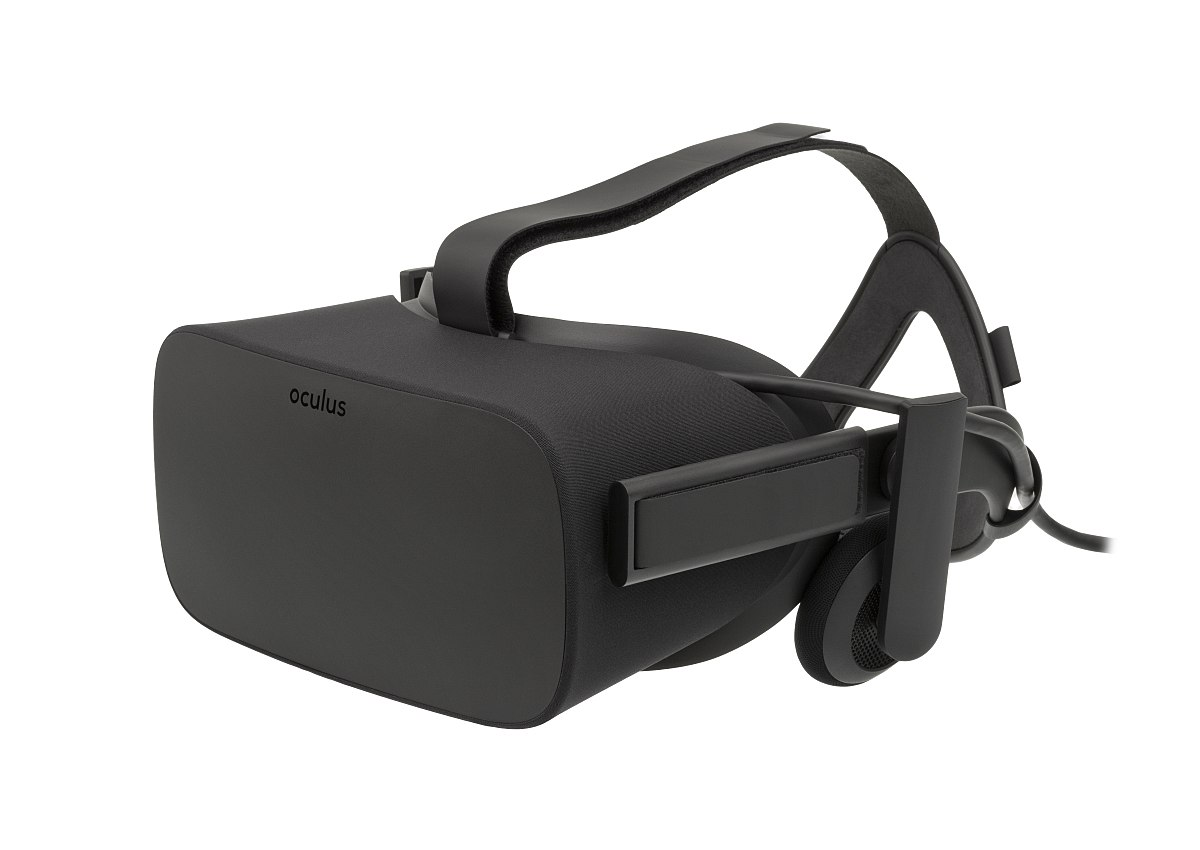
\includegraphics[width=0.7\linewidth]{img/1200px-Oculus-Rift-CV1-Headset-Front}
	\caption{Oculus rift head mounted display.}
	\label{fig:oculus}
\end{figure}

\begin{itemize}
	\item Accommodation-Vergence: As is reported in these \cite{disconfortReview}, \cite{vergenceDisconfort} articles the mismatch between accommodation and vergence in head mounted displays causes a conflict on the expected depths increasing the feeling of discomfort and dizziness.  One idea to reduce this effect is to dynamically move the position of screen frames as the focus changes from closer to distant objects and vice versa. To achieve this we will use a neuronal network that will be able to discern between closer and distant objects, also we will need the depth map obtained via the stereo camera setup. \\*
	In addition to this, a progressive change from one focus to the other may be needed, as a big change in focus can induce sickness to the user.
	
	\item Depth of field (DoF) blur: Recent investigations \cite{ifftConfortDoF} suggest that applying a DoF blur to a scene viewed using a head-mounted display can reduce visual discomfort, the challenge here is that our project has to make this DoF blur in real time in a real world environment, in contrast to the developed in that investigation where they used computer generated scenes. To achieve this we are going to use disparity map and the information obtained by a neural network that discerns between closer and distant objects.
\end{itemize} 

Thirdly, as the HDM will be used in workplaces, the idea of adding data to the environment, could improve the work-flow and the work efficiency. For this reason its think, that adding a third camera to the system can add valuable information that can be mixed with the environment. A similar idea can be found here \cite{vismerge} where a third camera is used to add information to the real world. For example with adding a infrared camera, the user can be warned by highlighting objects too hot to be touched.

Fourthly, as we discovered in a user testing done in the CVC \cite{unpublishCVC} last January, using a computer while wearing the HDM is a difficult task, mainly because the screen was unreadable for the brightness saturation of the image. For that reason a system capable of detecting computer screens and adapt the brightness, contrast and others parameters of the image stream will be developed.

Along all the development, user testing sessions will be taking place in order to check the improvements made between the different versions of the developed software and the different prototypes developed. The main goal of this sessions will be to evaluate if the developed software works and if it reduces the sickness feelings of the users. The procedure used in the user testing will be similar to the performed in \cite{ifftConfortDoF}, where the Simulator Sickness Questionnaire \cite{ssqQuestion} where used to evaluate the symptoms. 

A Objectives tree can be found in the figure \ref{fig:objective} in the appendix, it was done to recollect all the goals that this project want to achieve. As we will see in \ref{sec:planning}, not all of this goals will be reachable because of time constraints.

\section{Methodology}
Scrum and its variants are one of the most spread work methodologies nowadays.
The scrum methodology is the selected to be used in this project, however, as this project will only be done by one person, some changes have to be made. 

First as there is only one developer the daily meeting will be substituted with a weekly meeting with the stakeholders, in this case the tutor and the boss of the laboratory department in the CVC, in these meetings we will evaluate the development done, the issues faced that week and the problems solved. In addition to that we will discuss and review future milestones and the progress towards them.

Secondly, a backlog will be prepared at the beginning of the project and will contain the main goals divided in tasks, these tasks will be organized in groups of sprints easily done in a week. As each sprint has a backlog of task to be done, a tool can be used to organize this backlog, in this case Trello\cite{web:trello} will be used.

Thirdly, each iteration over the documentation and the development will be kept by a version tracker, in this case, github \cite{web:github} and its desktop client \cite{web:githubDesktop}. 

Keeping the main scrum methodology, I think it's interesting to grab some ideas from the Lean software development \cite{web:leanMethod}. The idea of removing the so called "Muda", non important extra features and processes, could be beneficial for this project because it could reach an overwhelming dimension for the limited time that is have.

%Another interesting idea from the lean method is  

Involving the tools that will need to be used develop the project, first of all, the current viewer version is made in C++ using the QT libraries \cite{web:qt}, therefore any tools that would be used need to be compatible with the current version of the viewer. For that reason, further investigation will be performed to identify which neural network library is more suitable.

\section{Planning}
\label{sec:planning}

\subsection{Dataset}
To be able to develop this project a dataset will be necessary to train the neural networks and to check the depth map. In this case as we have available three hardware prototypes, a data collection procedure will be possible and simple. For that reason a dataset caption session is planned.

Also a dataset will be used to make sure our dataset is correct and to encompass a broader range of environments. For that reason we selected first the Middlebury stereo dataset \cite{web:middelburyDataset} because it has a great dataset of stereo images and the groundtruth of their depth map. Additionally a dataset with indoor and outdoor scenes is recommended. Several dataset could be used with that purpose, for example the MIT's places dataset \cite{web:mitplaces} and the INDSECS indoors only dataset \cite{web:indecs}.

\subsection{Accommodation-Vergence}
\label{subsec:vergence}
In this stage, a neural network will be trained to detect the distance of the focus and the necessary vergence in the screen placement to help the user a more comfortable experience.
This will, alongside with the DoF blur, be the main time-consuming stage of the project and will have the following parts:
\begin{enumerate}
	\item \label{itm:preset}  Preset creation: In this task, the current viewer will be expanded with the creation of multiple and easy to change presets that will allow further user testing.
	
	\item \label{itm:UserTesting} User testing, presets: In this first user testing session after the finalization of task \ref{itm:preset}, the users will be told to configure their own focus settings and to try to change between them to adapt the focus to closer or distant objects. The goal here is to acknowledge whether the user feels better accommodation with the focus between objects.
	
	\item \label{itm:ProgressivePreset} Progressive preset change: After the development of \ref{itm:preset} and \ref{itm:UserTesting}, if the users report sickness because of the sudden change between presets, a smooth transition between them will be developed to reduce the issue. 
	
	\item Disparity map: In parallel with the development of the tasks \ref{itm:preset}, \ref{itm:UserTesting} and \ref{itm:ProgressivePreset}, a disparity map creator(matcher?) from a stereo pair is required to continue with further development. As this subject is complex per se and is not the main goal of this project, a library that already implements a good stereo matcher, like LIBELAS\cite{web:LIBELAS}, will be used. 
	
	\item Neural network with camera streams: This task will start after the analysis of the data collected in the task \ref{itm:UserTesting}, an the main goal will be to create a neural network capable of returning the value of the vergence. To achieve this several architectures will be tested and compared, with one, two or three streams from the cameras and including the disparity map information when developed.
	
	\item User testing: In this user session, the goal will be to check if the development done in this stage has reduced the sickness feelings of the users, and with which solution the user feel more comfortable.
\end{enumerate}

\subsection{Depth of field blur}
This stage will be developed after the finishing of the previous Accommodation-Vergence phase \ref{subsec:vergence} and shares some development with it. 

This problem can be resolved in to ways, using a disparity map only to create the DoF and using Neural network to aid the creation of it.

\begin{enumerate}
	\item Mock up blur: to ensure that the results of \cite{ifftConfortDoF} are applicable to real world scenarios, a mock up blur photo dataset will be made, and a user testing session will take place.
	
	\item Designing de pipeline: this task goal is to design, both pipelines, the disparity map only and the neural network aided.
	
	\item \label{itm:disparityversion} Disparity map version: this version will generate the DoF blur using only the disparity map to get the depth and using the center point of the cameras as the focus point.
	
	\item \label{itm:NNversion} Neural network adaptation: this task will take the neural network developed in the previous phase and will modify it to make it usable in this phase of the project. The idea is that this network will produce an indicative value of the blurriness needed using the camera images to determine whether the scene has closer or distant objects.
	
	\item User testing: Along with the development of \ref{itm:disparityversion} and \ref{itm:NNversion}, a user testing session will take place to check if this system has reduced the dizziness and which solution is more comfortable for the user.
\end{enumerate}

\subsection{Improving screen quality}
In this stage a system to improve the quality when the user is looking a screen will be developed. This system can be split in two tasks:
\begin{enumerate}
	\item \label{itm:QualityImprovements} Quality improvements: In this task a system capable of changing contrast, brightness and other image parameters will be developed, this system will not be automatic and will need the interaction of the user.
	
	\item Automatic switching: The goal of this task will be to free the user from the interaction with the system developed in task \ref{itm:QualityImprovements}, to achieve this a neural network will be developed to detect when a user is looking a screen.
\end{enumerate}

Part of the development of this objective will be left to future projects because of time constrains.

\subsection{Third camera}
This stage will have as a main goal the integration of a third camera in the viewer software and highlighting relevant information obtained using the third camera on stream viewed by the user. It can be split in the following tasks.

\begin{enumerate}
	\item \label{itm:Integration} Integration with the viewer: Introducing a third camera in the system will mean making some modifications in part of the viewer code. The goal of this task will be to prepare the different modules of the viewer for the introduction of the third camera.
	
	\item Research mixture: After the development of task \ref{itm:Integration}, a system to allow the mixture of images between visible and the third camera spectrum will be developed, the goal will be to add information to the user from the third camera different spectrum.
\end{enumerate}

Part of the development of this objective will be left to future projects because of time constrains.


\subsection{Research, documentation and planning}
This stage of the project can be split in two parts:
\begin{enumerate}
	\item Initial documentation: the documentation process will start at the beginning of the project and it includes, recollect information about the state of the art, do the planning and search about the different technologies involved in this project. 
	
	\item Progress documentation: this will be written along all the project and will consist in document every change and issue that can happen. When a part of the project changes its orientation or a milestone is achieve the documentation will be updated with the changes. 
	
	\item Closure documentation: When the project will approach the finish, an article, a recompilation of all the work done and a presentation will be made to wrap up the project.
	
\end{enumerate}

The general planning timeline can be found in the Gantt diagram figure \ref{fig:gantt} in the appendix.

\section{Acknowledgment}
This work is supported in part by a CVC transfer project with ProCare Light company, and partially funded by the Spanish Ministry of Economy and Competitiveness and FEDER under grants TIN2014-56919-C3-2-R and TIN2017-89723-P.

\bibliography{biblio}
\bibliographystyle{plain}

\appendix

\section*{Appendix}
\begin{figure}
	\begin{forest}
		for tree={%
			folder,
			l sep=0.6cm,
			grow'=0,
			fit=band,
		}
			[HDM
				[Modular HDM Viewer
				[Preset Shortcuts]
				[Better program configuration]
			]
			[Accommodation-Vergence
				[Preset creation]
				[Neural network]
				[Disparity map]
				[User testing]
			]
			[Depth of field blur
				[Mock-up blur]
				[Disparity map Version]
				[Neural network Version]
				[User testing]
			]
			[Third eye]
			[Screen quality]
		]
	\end{forest}
\caption{Objective Tree of the project}
\label{fig:objective}
\end{figure}

\begin{landscape}
	\begin{figure}
		\centering
		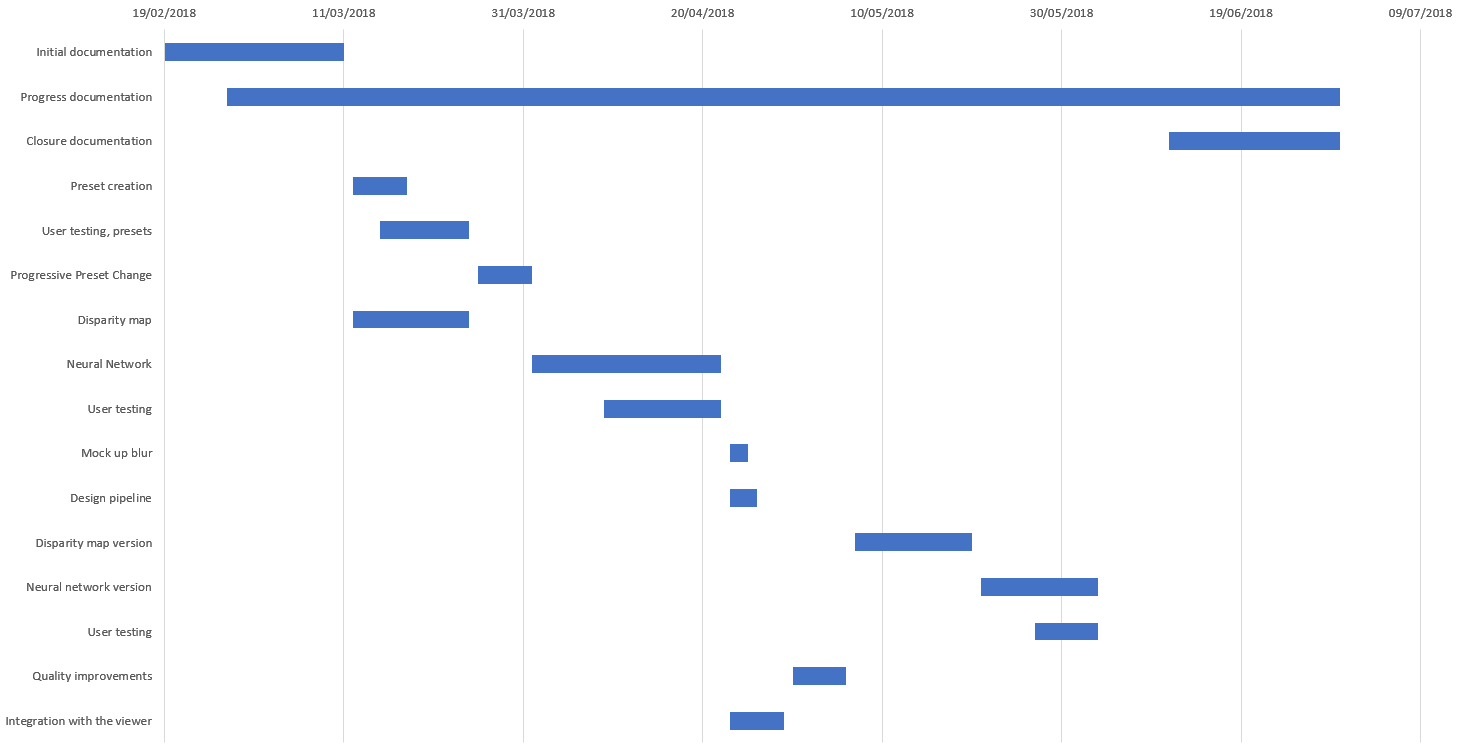
\includegraphics[width=1\linewidth]{img/gantt}
		\caption{Gantt diagram of the project.}
		\label{fig:gantt}
	\end{figure}

\end{landscape}




\end{document}

